% =====================================================================
%  Submission draft formatted for the American Economic Review (AER)
%  AER guidelines: PDF; 11- or 12-pt font, 1.5 spacing, 1-inch margins;
%  abstract of 100 words or fewer; about 40-45 pages; Chicago author-date
%  references; a separate Disclosure Statement for EACH coauthor;
%  compliance with the AEA Data and Code Availability Policy.
%  Build:  latexmk -pdf main.tex        (Overleaf: upload the folder)
%  [TODO] notes print in red and [Source] notes in blue while \drafttrue.
% =====================================================================
\documentclass[11pt]{article}

\usepackage[margin=0.9in]{geometry}
\usepackage[T1]{fontenc}
\IfFileExists{lmodern.sty}{\usepackage{lmodern}}{}
\usepackage{amsmath,amssymb}
\usepackage{graphicx}
\usepackage{placeins}
\usepackage{booktabs,threeparttable,multirow}
\usepackage{caption,subcaption}
\usepackage{setspace}
\usepackage{xcolor}
\usepackage[round,authoryear]{natbib}
\usepackage[colorlinks=true,linkcolor=black,citecolor=blue!50!black,urlcolor=blue!50!black]{hyperref}

\graphicspath{{figures/}}
\captionsetup{font=footnotesize,labelfont=bf,labelsep=period,skip=4pt}
\setstretch{1.0}
\setlength{\textfloatsep}{10pt plus 2pt minus 2pt}
\setlength{\floatsep}{8pt plus 2pt minus 2pt}
\setlength{\intextsep}{8pt plus 2pt minus 2pt}

% ---- AER-style numbering: I., II., ...; A., B., ... -------------------
\renewcommand{\thesection}{\Roman{section}}
\renewcommand{\thetable}{\arabic{table}}
\renewcommand{\thefigure}{\arabic{figure}}

% ---- draft notes -----------------------------------------------------
\newif\ifdraft \drafttrue
\newcommand{\todo}[1]{\ifdraft{\color{red!70!black}\small\textsf{[TODO: #1]}}\fi}
\newcommand{\source}[1]{\ifdraft{\color{blue!60!black}\footnotesize\textsf{[Source: #1]}}\fi}

\newcommand{\ES}{\textsc{es}}
\newcommand{\NQ}{\textsc{nq}}
\newcommand{\ZN}{\textsc{zn}}
\newcommand{\ZT}{\textsc{zt}}
\newcommand{\YM}{\textsc{ym}}
% ---- Outline numbering: unnumbered parts (Sensibility, Data, ...), I., II. inside each part,
%      A., B. below that. \ref to a subsection prints e.g. "Model, Section I".
\setcounter{secnumdepth}{3}
\renewcommand{\thesubsection}{\Roman{subsection}}
\renewcommand{\thesubsubsection}{\Alph{subsubsection}}
\makeatletter
\newcommand{\secname}{}
\renewcommand{\@seccntformat}[1]{\csname the#1\endcsname.\quad}
\renewcommand{\p@subsection}{\secname, Section~}
\renewcommand{\p@subsubsection}{\secname, Section~\thesubsection.}
\newcommand{\papersection}[2]{%
  \section*{#1}\phantomsection\addcontentsline{toc}{section}{#1}%
  \renewcommand{\secname}{#1}\def\@currentlabel{#1}\label{#2}%
  \setcounter{subsection}{0}}
\makeatother
\renewcommand{\thesubsection}{\Roman{subsection}}

\begin{document}

% ======================= title page ====================================
\begingroup
\begin{center}
{\Large\bfseries Surprises, Shapes or Machines?\\[4pt]
\large Forecasting the Market's Response to Macroeconomic Releases with Dynamic Time Warping (DTW)\par}
\vspace{1.5em}
{\large Benjamin Steel, Reza Zamani, Jack Duncan, Aaryen Mehta and Hoshea Zeng\footnote{%
Steel: BlackRock (email: \href{mailto:Benjamin.Steel@blackrock.com}{\nolinkurl{Benjamin.Steel@blackrock.com}}).
Zamani: Haas School of Business, University of California, Berkeley (email:
\href{mailto:rezazamani@berkeley.edu}{\nolinkurl{rezazamani@berkeley.edu}}).
Duncan: Haas School of Business, University of California, Berkeley (email:
\href{mailto:jack_duncan@berkeley.edu}{\nolinkurl{jack_duncan@berkeley.edu}}).
Mehta: Haas School of Business, University of California, Berkeley (email:
\href{mailto:aaryen@berkeley.edu}{\nolinkurl{aaryen@berkeley.edu}}).
Zeng: Haas School of Business, University of California, Berkeley (email:
\href{mailto:zenghaotian2@berkeley.edu}{\nolinkurl{zenghaotian2@berkeley.edu}}).
This paper grew out of a
BlackRock industry project in the Berkeley MFE program. We thank Ian Kaufman and Chris Pohalski
(Haas School of Business) for coordinating the project. This paper represents the views of the
authors only. It does not represent the views of BlackRock, Inc.\ or of the University of
California, Berkeley.}\par}
\vspace{0.5em}
{\normalsize Draft: September 2026\par}
\end{center}
\vspace{1.5em}

\begin{abstract}
\noindent
% AER: 100 words or fewer.
Do past market reactions to scheduled macroeconomic releases help forecast the next move? We
match the price path around each release to earlier paths with dynamic time warping (DTW) and
trade the move that followed the closest matches in four futures markets: the S\&P 500 (\ES),
Nasdaq-100 (\NQ) and Dow (\YM) equity indices and the 10-year Treasury note (\ZN).
The dispersion of the matches predicts the size of the next move; their direction is
weaker and changed sign around 2018. On 2021--2026 the \ES\ book earns a Sharpe ratio of 0.64
after costs with no market beta, \NQ\ only 0.11, and \YM\ loses ($-0.39$). The DTW book diversifies surprise-based
trading. \ZN\ reacts, but its tick size absorbs the edge.
\end{abstract}

\medskip
\noindent\textbf{JEL:} G14, G13, C14, E44\\
\noindent\textbf{Keywords:} dynamic time warping; analogue forecasting; macroeconomic
announcements; futures; event-driven trading; transaction costs


\endgroup
\vspace{0.5em}

\papersection{Introduction}{sec:intro}

Scheduled macroeconomic releases are among the cleanest information events in financial markets.
Their timing is announced months in advance, and futures prices react within the first minute
\citep{Fleming1999, Balduzzi2001, Andersen2003}. In equity-index futures, however, part of the
move continues well after that minute: after a hot CPI print the E-mini S\&P 500 (\ES) falls about
37 basis points (bps) in the first minute and a further 17 bps over the next half hour. This paper
asks whether the \emph{shape} of the market's reaction to a release, compared with its reactions
to earlier releases, forecasts that next move.

We match the price path around each release to past paths with dynamic time warping (DTW) and
trade the move that followed the closest matches. The book trades five back-to-back 30-minute
windows after every release that moves the market, enters only after the release is public, and
is scored on the held-out years 2021--2026 after costs in four futures markets: the S\&P 500 (\ES),
Nasdaq-100 (\NQ) and Dow (\YM) equity indices and the 10-year Treasury note (\ZN).

Three findings stand out. First, the dispersion of the matches forecasts the size of the next
move in every market and year, while their direction is weak and changed sign around 2018.
Second, the \ES\ book earns a Sharpe ratio of 0.64 at a quarter tick per side with no market beta,
but \NQ\ earns only 0.11 and \YM, added later as an out-of-sample market, loses ($-0.39$). Third,
the edge is concentrated in the first window after the release, and in \ZN\ it is smaller than
one tick. The Sensibility part explains the approach, the Data and Model parts describe the inputs
and the strategy, and the Backtest part reports the results.

\papersection{Sensibility}{sec:sense}

Markets rarely react to the same news on the same clock. The shape of the repricing repeats, but
the timing may differ by a few minutes from one release to the next. A distance metric that cannot
see through that slippage will call two identical reactions different. Dynamic time warping (DTW)
measures the similarity between two time series while letting their time axes stretch and
compress, so two paths are close if they trace the same shape, even when one runs faster or lags
the other \citep{Sakoe1978, Berndt1994}. This feature makes DTW well suited to price data:
Euclidean distance compares minute by minute, and correlation is just as rigid in time. We use
DTW as an analogue forecaster \citep{Lorenz1969}. We rank historical price paths by their
similarity to a target window and read off the returns that followed. We posit that similar price
paths have similar short-term forward returns. Figure~\ref{fig:dtw} illustrates the alignment.

\begin{figure}[!tb]
  \centering
  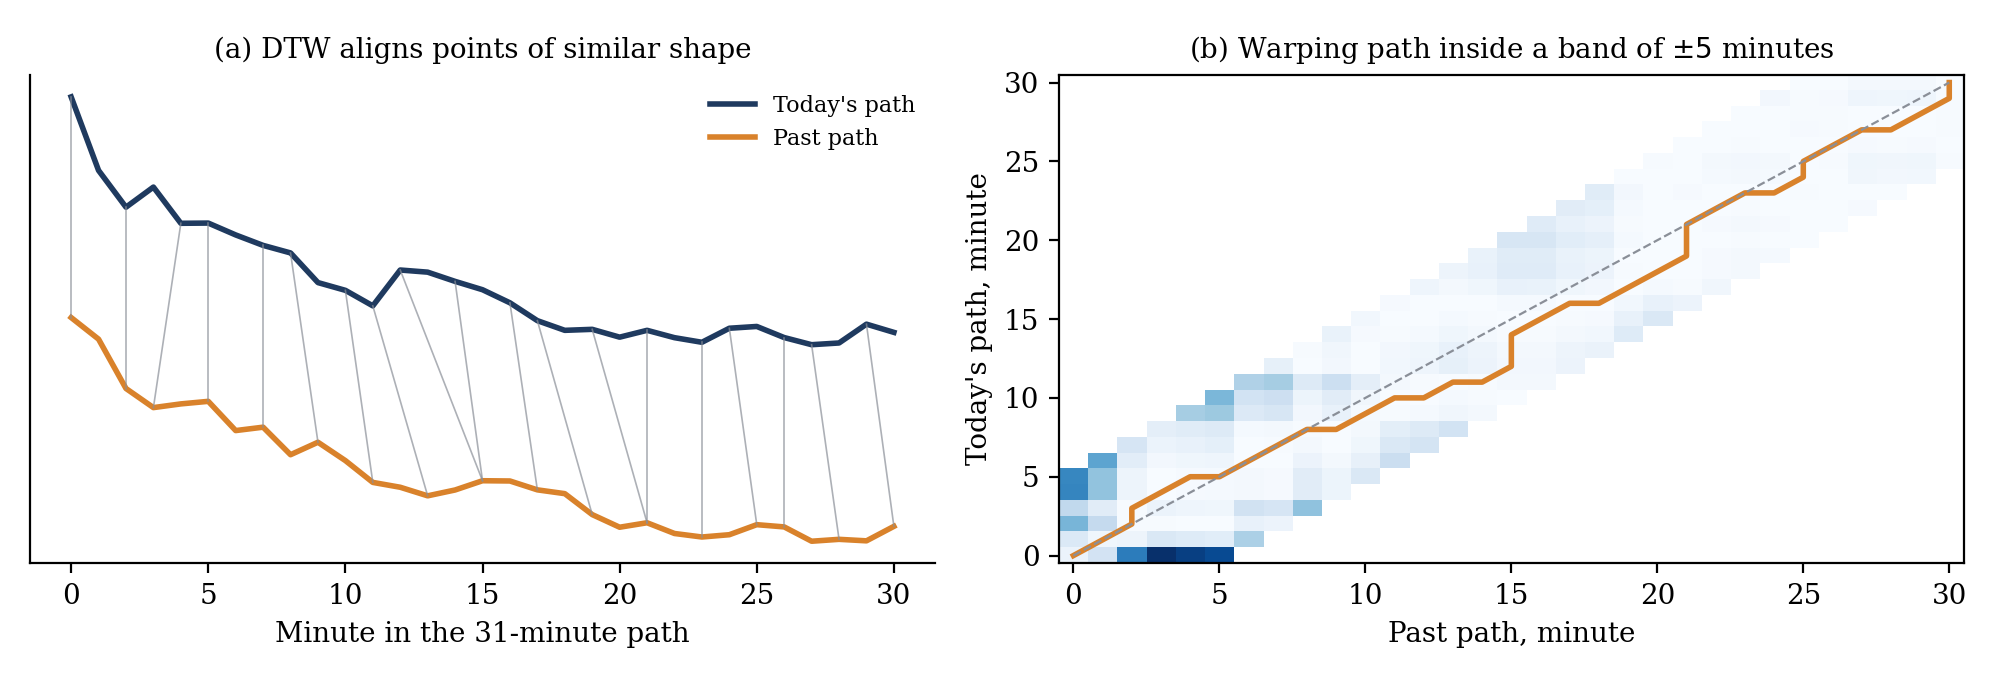
\includegraphics[width=0.6\linewidth]{dtw_illustration}
  \caption{How DTW compares two price paths (stylized example). Panel (a): the lines connect the
  points that DTW aligns; the past path reaches the same low about two minutes later. Panel (b):
  the local cost inside the band $|i-j|\le 5$ and the optimal warping path (orange); the dashed
  diagonal is the minute-by-minute (Euclidean) alignment.}
  \label{fig:dtw}
\end{figure}

Applied naively, DTW runs into two problems. The first is cost: comparing a target against every
window in years of minute-level data is slow. The second is that, with a large enough library,
some historical paths will match the target by pure luck, and a lucky match says nothing about why
the path formed. We address both issues by restricting the library to windows that follow
scheduled macroeconomic releases such as CPI and the Jobs Report, events macro traders reliably
react to. The library shrinks, and every match shares a common root: one public shock at a known
time, with participants repricing rate expectations together. Our refined hypothesis is that
similar price paths following scheduled macro releases have similar short-term forward returns.
For example, take the price path following a CPI release. Compared against past paths following
other releases, such as the Jobs Report, retail sales or PCE, most will strongly differ, yet a
few will trace nearly the same shape. Those few are far more likely to reflect the same
repricing than sheer luck.

\papersection{Data}{sec:data}

\subsection{Bloomberg macroeconomic events}\label{sec:bbg}

The event calendar is the Bloomberg U.S.\ economic release calendar from 2010 to 2026. It
contains 179 release lines---a line is one published statistic, such as ``CPI MoM'' or ``Change
in Nonfarm Payrolls''---and 27,137 release rows, each with the release date and time in Eastern
Time, the actual value and the median of the Bloomberg survey of forecasters. Most price and
labor-market data are released at 08:30, survey indicators such as the ISM indices at 10:00,
and FOMC decisions at 14:00.

The DTW model uses the calendar for its timing, not its values: a release is an instant $T$ at
which information arrives, and the model compares the market's reaction at $T$ with its reactions
at earlier releases. The actual values and the consensus are not used.

Many lines are released together as parts of one report. The CPI report alone produces eight
lines at the same second, and the Employment Situation report twelve. Trading each line
separately would trade the same minute several times, so \ref{sec:universe} groups the
lines into release families before any other step. In the family construction, 163 lines
collapse into 67 families.

\subsection{Futures data (S\&P 500, Nasdaq-100, Dow, 10-year and 2-year notes)}\label{sec:futures}

We use one-minute OHLCV bars from Databento (CME Globex, \texttt{GLBX.MDP3}) from July 2010 to
June 2026. Table~\ref{tab:contracts} summarizes the contracts. \ES, \NQ\ and \YM\ are continuous
front-month series rolled on the calendar; \ZN\ is rolled on volume. For \ES, the first years of
the vendor file had many incomplete sessions, and we re-pulled 2010--2015 so that the whole
sample has complete sessions. \YM\ (\$5 per index point, tick one point) is the only other
U.S.\ equity-index future on the same feed with one-minute history from 2010. Its file has 5.2
million one-minute bars; cleaning keeps 3,754 sessions (84--95\% of each year's sessions), and
4.8\% of the kept minutes are filled with the last price, 8--15\% before 2016, like early \NQ,
and under 2\% from 2018.

\begin{table}[!tb]
  \centering\footnotesize
  \caption{Contracts.}\label{tab:contracts}
  \begin{threeparttable}
  \begin{tabular}{lccccc}
    \toprule
    & \ES & \NQ & \YM & \ZN & \ZT \\
    \midrule
    Underlying & S\&P 500 & Nasdaq-100 & Dow Jones Ind. & 10-year note & 2-year note \\
    Continuous series & calendar roll & calendar roll & calendar roll & volume roll & --- \\
    Tick size & 0.25 points & 0.25 points & 1 point & 1/64 point & --- \\
    Value of one point & \$50 & \$20 & \$5 & \$1,000 & --- \\
    Value of one tick & \$12.50 & \$5.00 & \$5.00 & \$15.625 & --- \\
    One tick, in bps of contract value & $\approx 0.5$ & $\approx 0.1$--$0.3$ & $\approx 0.25$--$1$ & $\approx 1.4$ & --- \\
    Role in this paper & traded & traded & traded & cost-gated & dropped \\
    \bottomrule
  \end{tabular}
  \begin{tablenotes}\footnotesize
    \item Notes: Databento \texttt{GLBX.MDP3}, one-minute bars, July 2010 to June 2026.
    \ZT\ was pulled but dropped: before 2019, fewer than 7\% of its release windows have a
    trade in every minute, and a check against tick-level trades confirmed that the gaps are
    minutes without trading, not missing data.
  \end{tablenotes}
  \end{threeparttable}
\end{table}

\paragraph{Sessions.} A trading session runs from 18:00 to 17:00 Eastern Time and is dated by
the day on which it closes. We drop exchange holidays and keep a session only if it has at least
85\% of the asset's median number of bars per weekday session in that year; the threshold is
relative because \ZN\ and early \NQ\ and \YM\ trade fewer minutes than \ES. Minutes without a trade inside
a kept session are filled with the last price. Bars are labelled by their start: the bar
labelled 08:30 covers 08:30:00--08:30:59.

\paragraph{Rolls.} A path or trade that straddles a change of contract would include the
calendar-spread jump. We drop any game in which the contract changes between the first minute
of its path and its exit, and buy-and-hold benchmarks skip the price jump at each roll.

\begin{figure}[!tb]
  \centering
  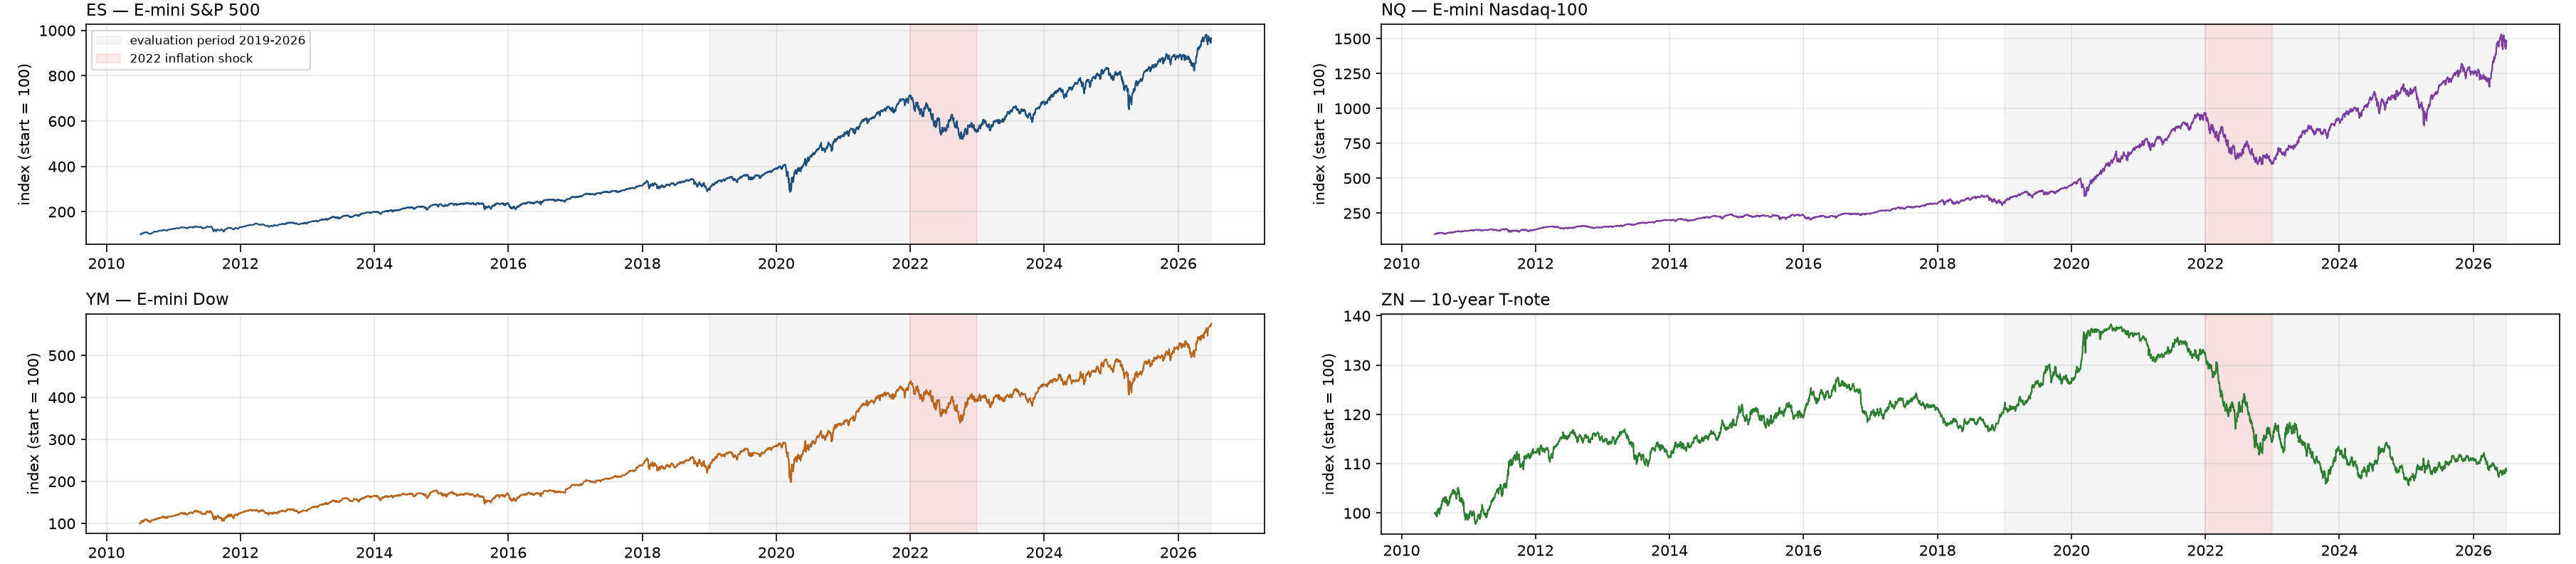
\includegraphics[width=\linewidth]{fig01_markets_overview_2x2}
  \caption{\ES, \NQ, \YM\ and \ZN, 2010--2026. Roll-adjusted daily prices rebased to 100. Grey: the
  2019--2026 period; red: the 2022 inflation shock.}
  \label{fig:markets}
\end{figure}

Figure~\ref{fig:markets} shows the equity and Treasury futures over the sample, including \YM.

\subsubsection{Why we chose to look at these}\label{sec:why_assets}

All five contracts are among the most liquid futures in the world, trade nearly around the clock
on CME Globex, and react to the same U.S.\ releases, so one calendar and one session definition
serve them all. They differ in how they should react. A hot inflation print raises the expected
path of the policy rate and lowers the present value of future earnings, more so for the
long-duration technology stocks that dominate \NQ; the Dow behind \YM\ holds fewer technology and
more industrial and financial stocks than the S\&P 500, so it tests whether what works in \ES\
carries to a different mix of the same market. The Treasury notes respond to the same news through
yields: the CPI surprise explains about 30\% of the five-minute reaction of \ZN, as it does for
\ES. What separates the markets for a strategy that trades often is the tick: one tick is about
0.5 bps of contract value in \ES, 0.1--0.3 bps in \NQ\ and 0.25--1 bp in \YM, but about 1.4 bps in
\ZN, large next to its 30-minute moves. \ES\ and \NQ\ are the core of the book; \YM\ was added after
their results were known, as an out-of-sample market; \ZN\ is a candidate that a cost gate admits
or excludes (\ref{sec:gating}).

\subsubsection{Why we dropped the 2-year}\label{sec:why_zt}

The 2-year note future (\ZT) is the most direct read on the expected policy rate and would be the
natural market for rate news. But a path-based method needs a price in every minute of the path,
and before 2019 fewer than 7\% of \ZT's release windows have a trade in every minute. A fresh
pull compared against tick-level trades matched exactly, so the gaps are minutes in which \ZT\ did
not trade, not missing data. With a library that sparse before 2019, the analogues cannot be
built, so we dropped \ZT\ at the data stage.

\subsection{Data for DTW: the event panel}\label{sec:dtwdata}

The DTW model does not use the bars directly. It uses a panel of \emph{games} built from them, one
row for each asset, release family, release time and window (\ref{sec:universe}, \ref{sec:five}).
Each row carries three objects, all taken from the cleaned one-minute closes of
\ref{sec:futures}:
\begin{itemize}\itemsep0pt
  \item \textbf{The path:} the 31 closes ending at the entry minute, standardized within the
  window (equation~\eqref{eq:path}). For the first window the path ends at $T+1$, so it holds the
  last half hour before the release and the first minute of the reaction.
  \item \textbf{The target:} the log return from the close of the entry minute to the close 30
  minutes later, the return that the trade earns.
  \item \textbf{The labels:} the family, the clock slot, the window, the contract and whether the
  family passes the impact screen in that year (the \emph{admitted} flag).
\end{itemize}
A game is kept only if every minute of its path and of its holding window is inside a kept session,
the release minute and the minute after it have a price, and the same contract is traded from the
first minute of the path to the exit. A missing minute is never interpolated; the game is dropped.
The release times come from the Bloomberg calendar (\ref{sec:bbg}), after the 163 release lines
are grouped into 67 families.

Every game, admitted or not, enters the library of candidate analogues; only admitted games are
traded. The library is therefore much larger than the traded set: on \ES\ there are about 57,000
games in 2010--2026 but 3,420 admitted ones (Table~\ref{tab:panel}). The first three years,
2010--2012, are a burn-in period: they fill the library and give the impact screen its 30 earlier
releases, but no game in them is scored. The DTW features are computed for admitted games only,
from strictly earlier games in the library, so the panel can be built once and then split by year
into the training, validation and test samples of \ref{sec:whattest}. The panel for the four
assets has 223,583 rows.

\begin{table}[!tb]
  \centering\footnotesize
  \caption{The DTW event panel, 2010--2026.}\label{tab:panel}
  \begin{threeparttable}
  \begin{tabular}{lrrrr}
    \toprule
    & \ES & \NQ & \YM & \ZN \\
    \midrule
    Clean one-minute bars (millions) & 5.39 & 5.26 & 5.20 & 5.39 \\
    Games, all 67 families & 57,146 & 55,317 & 54,455 & 56,665 \\
    Families admitted in some year & 8 & 8 & 5 & 12 \\
    Admitted games with DTW features & 3,420 & 2,735 & 2,390 & 5,420 \\
    \quad of which scored in training, 2013--2017 & 820 & 525 & 640 & 1,085 \\
    \quad of which scored in validation, 2018--2020 & 840 & 665 & 460 & 1,130 \\
    \quad of which in the test years, 2021--2026 & 1,760 & 1,545 & 1,290 & 3,090 \\
    Trades in the test years, 2021--2026 (after the gate) & 1,202 & 1,141 & 870 & 1,945 \\
    Median analogue dispersion $\sigma_e$ (bps) & 17.8 & 24.1 & 17.0 & 6.1 \\
    \bottomrule
  \end{tabular}
  \begin{tablenotes}\footnotesize
    \item Notes: A game is one (asset, family, release, window). All games form the library of
    candidate analogues; admitted games are those whose family passes the impact screen in that
    year, and only they are traded. Trades in the test years are admitted games that pass the gate
    of equation~\eqref{eq:gate}, after games at the same minute are merged.
  \end{tablenotes}
  \end{threeparttable}
\end{table}

The panel is small where it matters. Training scores 820 \ES\ games and validation 840, and the
signal we look for is a correlation of a few hundredths; this is why the setting is fixed in
advance and checked once (\ref{sec:robust}). The panel is also uneven across assets: the impact
screen admits more families on \ZN, because the Treasury market reacts to more of the calendar, and
\ZN's analogues disagree by a third as much as \ES's in bps, in line with its smaller moves. \YM\ has the
fewest admitted families: CPI, payrolls, the ISM Manufacturing and Services indices and the FOMC
Minutes, the core of the \ES\ list without Core PCE, Retail Sales and Wholesale Inventories.

\papersection{Model}{sec:model}

The model decides which releases to trade (\ref{sec:universe}), turns the price path at entry into a
forecast (\ref{sec:signal}) and turns the forecast into positions (\ref{sec:strategy}). Nothing in it
uses data at or after the entry minute.

\subsection{Event Universe Construction}\label{sec:universe}

Release lines that share at least 80\% of their timestamps are grouped into one \emph{family}, so
each report (CPI, the Employment Situation) is one event. A family is admitted for asset $a$ in year
$y$ if it moves the market more than other releases at the same clock slot. With
$m_T=|p_{T+30}-p_T|$ the absolute 30-minute move after minute $T$,
\begin{equation}\label{eq:impact}
  I_{f,a,y}=\overline{m}_{T\in\mathcal{R}_f}\big/\,\overline{m}_{T\in\mathcal{C}_f},
\end{equation}
where $\mathcal{R}_f$ are the family's earlier releases and $\mathcal{C}_f$ the same clock slot on
days when another family releases there but $f$ does not. A family needs 30 earlier releases and a
Welch $t$-statistic of at least 2 on the log moves; the screen is redone each year from earlier years
only. On \ES\ it admits eight families (payrolls, CPI, ISM Manufacturing and Services, FOMC Minutes,
Retail Sales, Core PCE, Wholesale Inventories). The FOMC decision fails, because at 14:00 its only
control is the Minutes. Each admitted release is traded in five windows; one (asset, release,
window) is a \emph{game}.

\subsection{Signal}\label{sec:signal}

For game $e$ with entry minute $\tau_e$, the path is the 31 log prices ending at entry, standardized,
\begin{equation}\label{eq:path}
  q_{e,i}=(p_{\tau_e-31+i}-\bar p_e)/s_e,\qquad i=1,\ldots,31,
\end{equation}
so DTW compares the shape of the reaction, not its size; the target is the next 30-minute return
$y_e$. Candidates are earlier games on the same asset, clock slot and window, from any family, that
exited before $e$ entered, within three years and at most the 600 most recent (at least 20 are
required). The DTW distance $d_j$ to each candidate uses squared local costs and a Sakoe--Chiba band of
five minutes \citep{Keogh2005}. The $K=15$ nearest neighbours $\mathcal{K}_e$ are weighted by
similarity and age $\alpha_j$ (days), $\omega_j\propto d_j^{-1}e^{-\alpha_j/730}$, and give two
features:
\begin{equation}\label{eq:features}
  \mu_e=\sum_{j\in\mathcal{K}_e}\omega_j y_j,\qquad
  \sigma_e=\Big(\sum_{j\in\mathcal{K}_e}\omega_j (y_j-\mu_e)^2\Big)^{1/2}.
\end{equation}
The mean $\mu_e$ forecasts the direction of the next move; the dispersion $\sigma_e$ measures how much
the analogues disagreed, and forecasts the move's size (\ref{sec:signalquality}). The setting was
chosen on \ES\ in an earlier version of the model and is used unchanged for the other assets.

\subsection{Model}\label{sec:strategy}

\subsubsection{How do we turn this signal into a strategy}

The position in game $e$ is a direction, a gate and a size,
$w_e=\operatorname{sign}(\mu_e)\,G_e\,S_e$, held for 30 minutes from the close of the entry minute.
Games of different families at the same minute are merged into one position. With $n$ ticks of
slippage per side, tick $\delta$ and entry price $P_e$, the net return in bps is
\begin{equation}\label{eq:cost}
  r_e=w_e y_e-|w_e|\cdot 2n\,\delta/P_e\times 10^4 ,\qquad n\in\{0,\tfrac14,\tfrac12\}.
\end{equation}

\subsubsection{Why 5 windows?}\label{sec:five}

Each release is traded in five back-to-back 30-minute windows entering at $T+a_k$,
$a_k\in\{1,31,61,91,121\}$ (Figure~\ref{fig:ladder}). The reaction to a large release lasts more
than 30 minutes; one window gives too few trades to measure a small edge (five give about 225 a year
in \ES); and the windows test where the information is: if the path carries news, the first window
should be best (\ref{sec:hitrate}). No window enters at $T$, whose price predates the release.

\begin{figure}[!tb]
  \centering
  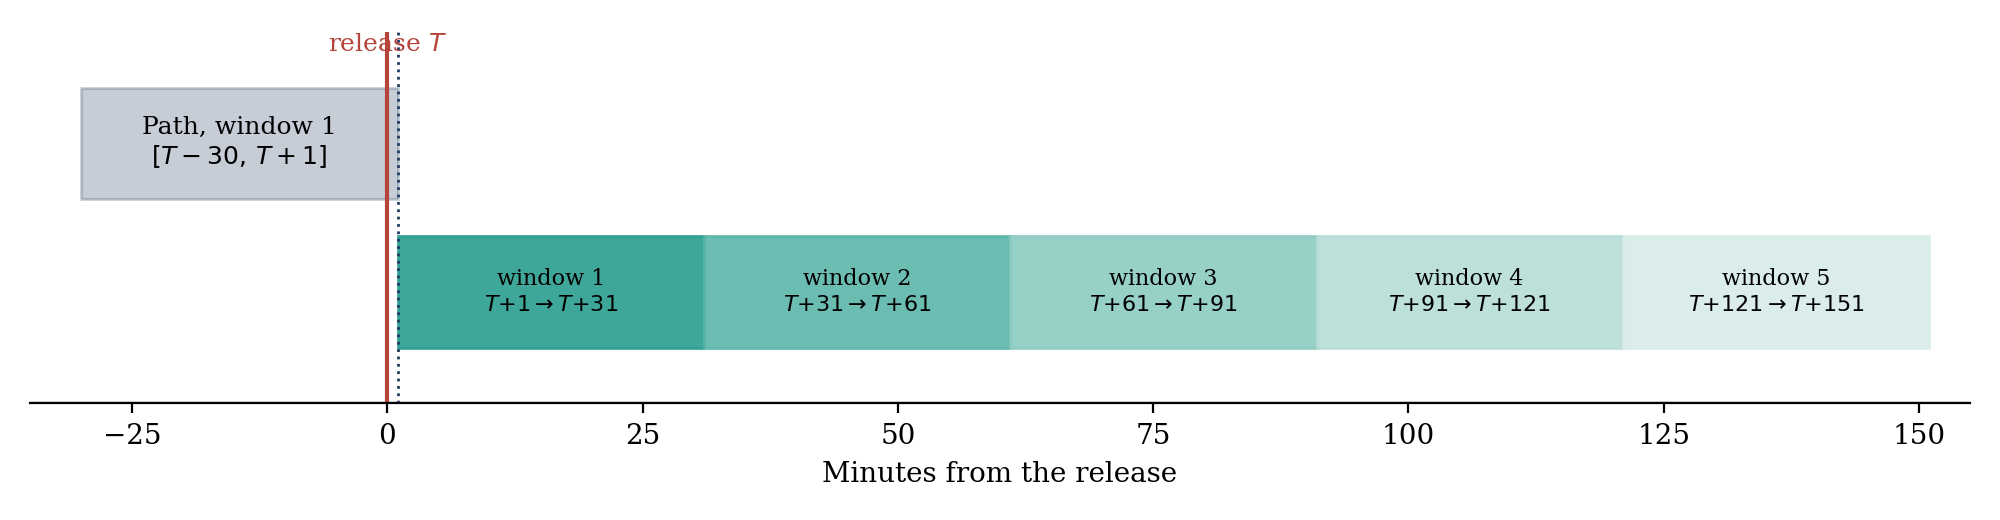
\includegraphics[width=0.48\linewidth]{event_ladder}
  \caption{The anchor ladder: five 30-minute windows after a release at $T$. Each window's path is
  the 31 minutes ending at its entry.}
  \label{fig:ladder}
\end{figure}

\subsubsection{Gating}\label{sec:gating}

The forecast is noisy near zero, so the book trades only its tails,
\begin{equation}\label{eq:gate}
  G_e=\mathbf{1}\{\mu_e\le Q_{0.3}\ \text{or}\ \mu_e\ge Q_{0.7}\},
\end{equation}
with quantiles fixed on the asset's 2013--2020 games: the outer 60\% of forecasts are traded.

\subsubsection{Weighting}

Trades are sized inversely to the dispersion, $S_e=\min(\tilde\sigma/\sigma_e,\,2)$, with
$\tilde\sigma$ its median in the fitting years: consistent analogues trade up to two contracts,
scattered ones less than one. Assets are combined with inverse-volatility weights reset monthly,
\begin{equation}\label{eq:assetweights}
  R_t=\sum_a\lambda_{a,t}R_{a,t},\qquad
  \lambda_{a,t}\propto G^{c}_{a,t}/\hat v_{a,t},
\end{equation}
where $\hat v_{a,t}$ is the 60-session volatility of the futures and $G^c_{a,t}$ a cost gate: an asset
is traded only while a round trip costs less than 10\% of its median 30-minute move on admitted
releases over the past year. \ES\ and \NQ\ always pass (weights about 58\% and 42\%), as does \YM\
(about 36/26/38\% with \ES\ and \NQ); \ZN\ passes only in part of 2023 (\ref{sec:treasury_result}).

\papersection{Backtest}{sec:backtest}

\subsection{What did we test}\label{sec:whattest}

We trade the model of the Model part, with its setting and rule fixed in advance, and score it on
the held-out years. Returns are in bps of one contract's notional, summed rather than compounded,
on a daily grid of trading sessions with zero on days without a trade; return, volatility and
the Sharpe ratio are annualized over 252 sessions. Costs are charged per side at a quarter or a
half tick.

\subsubsection{Time period}

\paragraph{Train, validation and test split.} Table~\ref{tab:split} shows how the years are used.
The first three years only fill the library of past reactions and the history the universe
screen needs. Settings are chosen on the training years, checked on the validation years, and
the test years are used to report results. The gate cut-offs and the size reference come from
2013--2020, so nothing in the test years is fitted.

\begin{table}[!tb]
  \centering\footnotesize
  \caption{Sample split.}\label{tab:split}
  \begin{tabular}{lll}
    \toprule
    Period & Years & Use \\
    \midrule
    Burn-in    & 2010--2012 & library of past reactions and screen history only \\
    Train      & 2013--2017 & choosing the DTW setting, gate and sizing \\
    Validation & 2018--2020 & checking that the choice holds \\
    Test       & 2021--2026 & results \\
    \bottomrule
  \end{tabular}
\end{table}

\paragraph{Why 30 minutes.} Each trade is held for 30 minutes and each path is the 31 minutes
ending at the entry. The horizon matches how long the news keeps moving prices: after hot CPI
prints \ES\ falls about 37 bps in the first minute and a further 17 bps by $T+30$, and is roughly
flat over the following half hour; \NQ\ and \YM\ behave the same way. A 30-minute path is long
enough to contain the whole first reaction and short enough that the library of past releases at
the same clock time holds hundreds of comparable paths. Equal path and holding lengths also make
the five windows of the ladder back-to-back, so no minute is traded twice.

\subsubsection{Assets}

Each asset is first traded on its own with the same setting, gate and sizing: \ES\ and \NQ, the
core of the book; \YM, run through the identical pipeline after the \ES\ and \NQ\ results were
known, as an out-of-sample market; and \ZN. Two multi-asset books follow.

\subsubsection{Equities book}

The equities book combines \ES\ and \NQ\ with the inverse-volatility weights and cost gate of
equation~\eqref{eq:assetweights}; both always pass the gate at a quarter tick, and the weights
average 58\% \ES\ and 42\% \NQ. We also report the three-index book \ES\ + \NQ\ + \YM, with
weights of about 36\%, 26\% and 38\%.

\subsubsection{Combined book}

The combined book adds \ZN\ on the same terms, and the cost gate decides whether it is traded.
Before costs every asset passes and \ZN\ takes about 60\% of the weight; at a quarter tick a round
trip is 10--17\% of \ZN's typical 30-minute move, so it is excluded except in part of 2023
(\ref{sec:treasury_result}).

\subsection{General Statistics}\label{sec:signalquality}

\paragraph{Signal quality.} Before trading, we ask whether the two features rank what happened
next (Figure~\ref{fig:ic}). The direction forecast $\mu$ ranks the next return
\emph{negatively} in the training years ($-0.060$ in \ES, $-0.042$ in \NQ) and \emph{positively}
in the validation years ($+0.069$ and $+0.091$); in \YM\ and \ZN\ it is close to zero in both
($-0.006$ and $+0.018$; $-0.003$ and $-0.005$). The dispersion $\sigma$, in contrast, ranks the
absolute size of the next move positively in every market and period, at 0.10--0.24. The
analogues know how large the next move will be; what they say about its direction is small and
changed sign around 2018.

\begin{figure}[!tb]
  \centering
  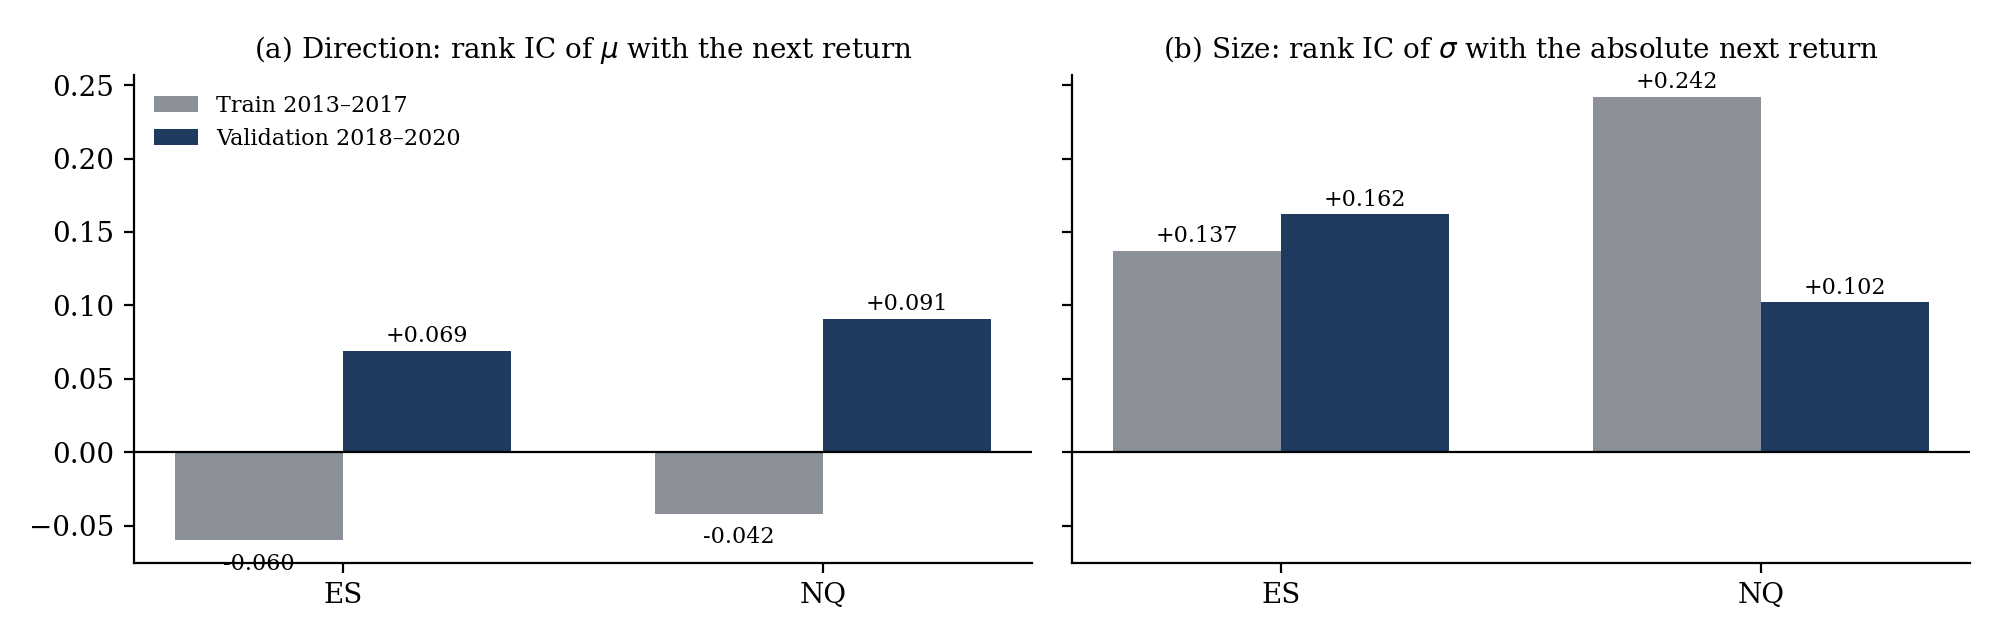
\includegraphics[width=0.55\linewidth]{dtw_ic}
  \caption{Information coefficients of the DTW features on admitted games, \ES\ and \NQ. Panel (a):
  rank correlation of $\mu$ with the next 30-minute return. Panel (b): rank correlation of $\sigma$
  with the absolute next 30-minute return.}
  \label{fig:ic}
\end{figure}

\paragraph{Results.} Table~\ref{tab:results} reports the test years. The \ES\ book trades 1,202
times, about 225 a year, and earns a Sharpe ratio of 0.78 before costs, 0.64 at a quarter tick and
0.49 at a half tick, against 0.69 for holding \ES, with a drawdown of $-5.0\%$ against $-31.1\%$
and a beta of 0.007. Half its trades win and 53\% are long, so it is not a disguised long
position. \NQ\ is positive but weak (0.11 at a quarter tick). \YM\ does not work: only five
families pass its screen, and it loses before costs ($-0.32$) and after them ($-0.39$). The
equities book earns 0.54 with a drawdown of $-5.3\%$; adding \YM\ lowers it to 0.27. The combined
book earns 0.40 (Figure~\ref{fig:sharpe}).

\begin{table}[!tb]
  \centering\footnotesize
  \caption{General statistics of the DTW event book, test years 2021--2026, quarter tick per side.}\label{tab:results}
  \begin{threeparttable}
  \setlength{\tabcolsep}{4pt}
  \begin{tabular}{lccccccccc}
    \toprule
    & & \multicolumn{3}{c}{Sharpe ratio} & Buy-and- & Total & Ann.\ & Max & Hit \\
    \cmidrule(lr){3-5}
    Book & Trades & Gross & $\tfrac14$ tick & $\tfrac12$ tick & hold & return & vol & DD & rate \\
    \midrule
    \ES & 1,202 & 0.78 & 0.64 & 0.49 & 0.69 & $10.9\%$ & 3.2\% & $-5.0\%$ & 50.0\% \\
    \NQ & 1,141 & 0.14 & 0.11 & 0.08 & 0.58 & $2.1\%$ & 3.6\% & $-8.2\%$ & 49.5\% \\
    \YM & 870 & $-0.32$ & $-0.39$ & $-0.47$ & 0.67 & $-4.8\%$ & 2.4\% & $-8.0\%$ & 50.0\% \\
    \ZN & 1,945 & 0.34 & $-0.97$ & $-2.24$ & $-0.69$ & $-7.4\%$ & 1.4\% & $-8.0\%$ & 46.9\% \\
    Equities (\ES\ + \NQ) & 2,343 & 0.66 & 0.54 & 0.42 & 0.65 & $7.4\%$ & 2.6\% & $-5.3\%$ & 49.8\% \\
    \ES\ + \NQ\ + \YM & 3,213 & 0.39 & 0.27 & 0.14 & 0.68 & $2.8\%$ & 2.0\% & $-3.0\%$ & 49.8\% \\
    Combined (\ES\ + \NQ\ + \ZN) & 2,476 & 0.76 & 0.40 & 0.41 & 0.24 & $5.4\%$ & 2.5\% & $-5.3\%$ & 49.3\% \\
    \bottomrule
  \end{tabular}
  \begin{tablenotes}\footnotesize
    \item Notes: Direction $\operatorname{sign}(\mu)$, outer 60\% of $\mu$ with cut-offs from
    2013--2020, size $\min(\tilde\sigma/\sigma,2)$, five windows per admitted release. Return,
    volatility, drawdown and hit rate at a quarter tick. Multi-asset books use the weights and
    cost gate of equation~\eqref{eq:assetweights}, so each cost column is the book a trader facing
    that cost would run. Buy-and-hold drawdowns: \ES\ $-31.1\%$, \NQ\ $-48.3\%$, \YM\ $-25.6\%$.
  \end{tablenotes}
  \end{threeparttable}
\end{table}

\begin{figure}[!tb]
  \centering
  \begin{subfigure}[b]{0.58\linewidth}\centering
    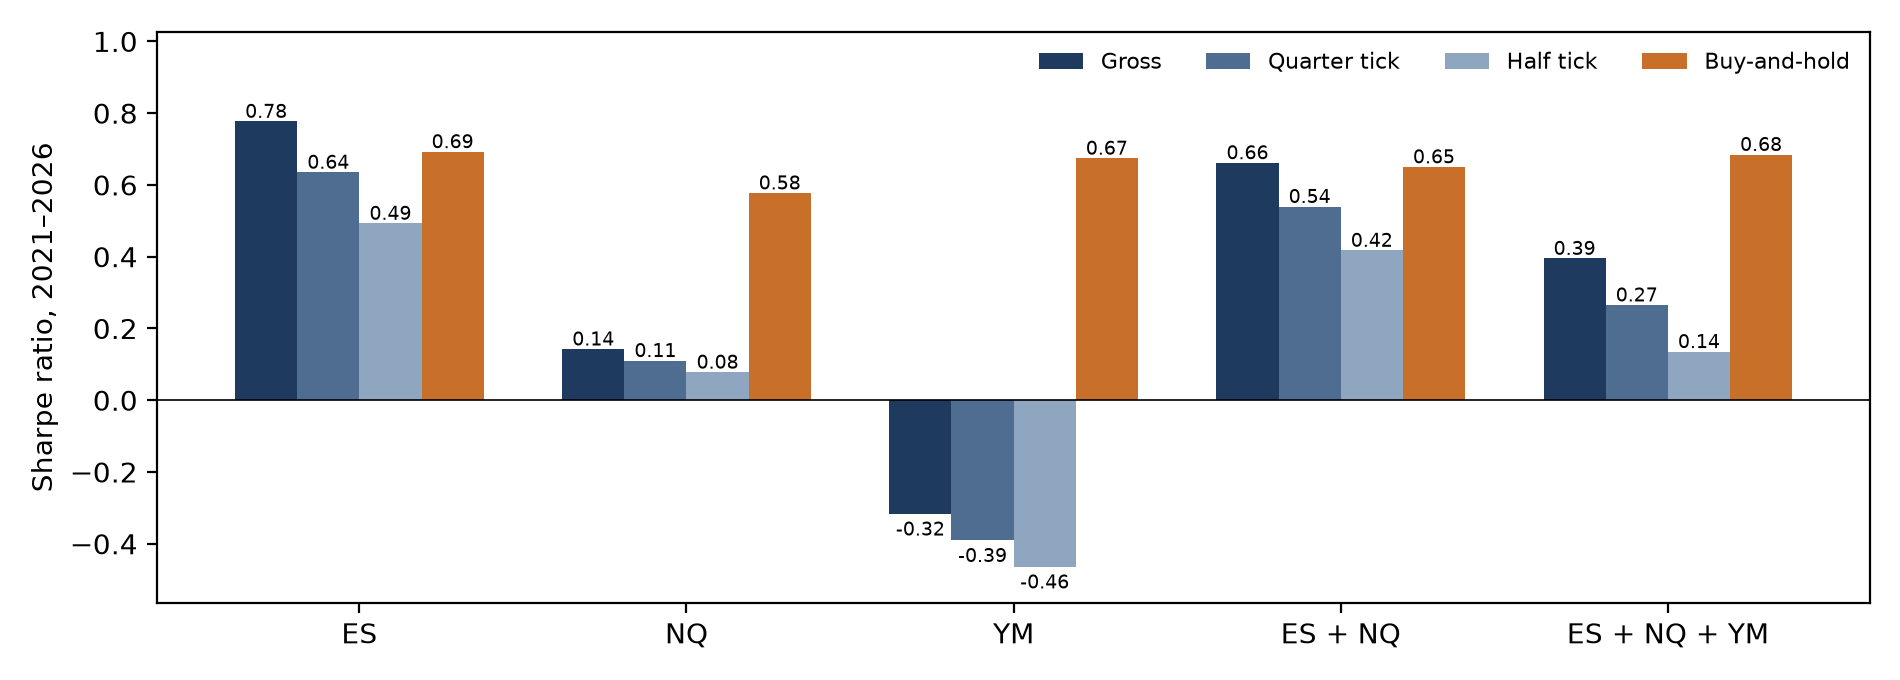
\includegraphics[width=\linewidth]{sharpe_by_cost_with_ym}
    \caption{Sharpe ratio by cost level, against buy-and-hold.}\label{fig:sharpe}
  \end{subfigure}\hfill
  \begin{subfigure}[b]{0.4\linewidth}\centering
    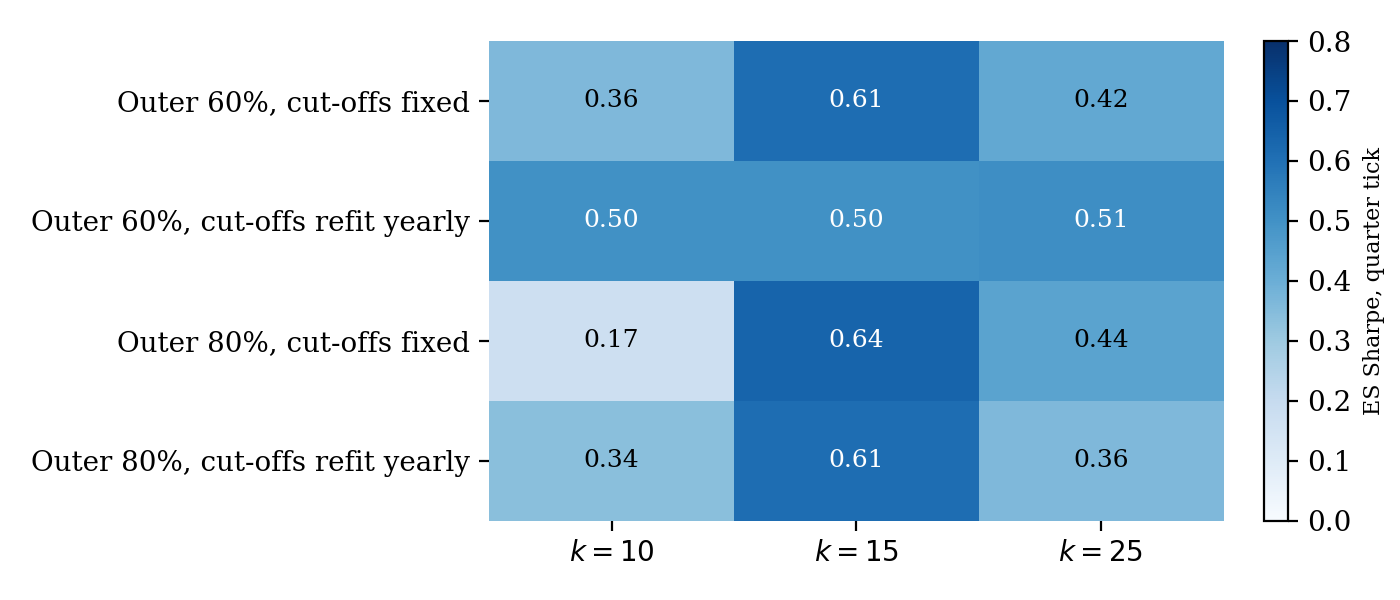
\includegraphics[width=\linewidth]{robustness_es}
    \caption{\ES\ Sharpe ratio at a quarter tick by $K$, gate width and cut-off rule.}\label{fig:robust}
  \end{subfigure}
  \caption{The DTW event book, 2021--2026. Panel (b): cut-offs are either fixed from 2013--2020
  or recomputed each year.}
  \label{fig:book}
\end{figure}

\paragraph{Checks.}\label{sec:robust} Table~\ref{tab:checks} reports five checks. Rebuilding the
features with the path running five minutes \emph{past} the entry raises the Sharpe ratio to
about 2.8 in every market, so the real book's timing is sound. Drawing the direction of each trade
at random beats the \ES\ book only 4.1\% of the time, but beats \NQ\ and \YM\ often ($p=0.37$ and
0.76). Holding the same windows always long loses in every book, so the \ES\ profit comes from
direction. \ES\ breaks even at 1.36 ticks per side. Across twelve gate, cut-off and sizing rules
\ES\ and the equities book are always positive, \YM\ only once, and across the number of
neighbours $K$ (Figure~\ref{fig:robust}) the \ES\ Sharpe ratio ranges from 0.17 to 0.64. Broader
searches over about 138,000 settings confirm that the direction is unstable across periods (the
Sharpe ratios of the same settings on 2014--2017 and 2018--2020 correlate at 0.15). The appraisal
ratio---alpha on buy-and-hold over residual volatility---is 0.61 for \ES\ and 0.53 for the
equities book; with a directional IC of 0.027 on about 225 bets a year, the fundamental law of
active management \citep{Grinold2000} implies about 0.4, so 0.4--0.6 is a fair range.

\begin{table}[!tb]
  \centering\footnotesize
  \caption{Checks on the DTW event book, 2021--2026, quarter tick per side.}\label{tab:checks}
  \begin{threeparttable}
  \begin{tabular}{lccccc}
    \toprule
    & \ES & \NQ & \YM & \ES\ + \NQ & \ES\ + \NQ\ + \YM \\
    \midrule
    Leak test: Sharpe with the path 5 minutes past entry & 2.86 & 2.85 & 2.84 & 3.62 & 3.83 \\
    Random-sign test: $p$-value, 5,000 draws & 0.041 & 0.37 & 0.76 & 0.064 & 0.18 \\
    Always long in the same windows: total return & $-2.4\%$ & $-1.0\%$ & $-6.2\%$ & $-1.8\%$ & $-3.6\%$ \\
    Break-even cost, ticks per side & 1.36 & 1.10 & --- & 1.35 & 0.76 \\
    Rules with Sharpe $>0$, of 12 & 12 & 7 & 1 & 12 & 12 \\
    Appraisal ratio vs buy-and-hold & 0.61 & 0.11 & $-0.38$ & 0.53 & 0.26 \\
    \bottomrule
  \end{tabular}
  \begin{tablenotes}\footnotesize
    \item Notes: \YM\ loses before costs, so it has no break-even cost. The \YM\ columns come from
    the same code run with \YM\ added, in which the \ES, \NQ\ and equities results reproduce exactly.
  \end{tablenotes}
  \end{threeparttable}
\end{table}

\subsection{Hit rate per window}\label{sec:hitrate}

Table~\ref{tab:window} and Figure~\ref{fig:byanchor} split the book by window. The first window,
entering at $T+1$, is the best in every equity index: it wins 53\% of its trades in \ES, 53\% in
\NQ\ and 58\% in \YM, with Sharpe ratios of 0.95, 0.38 and 0.41, against 1.7\%, 5.4\% and $-3.0\%$ for
always long in the same windows. The hit rate then falls toward a coin flip in the second to
fourth windows, and the fifth, at $T+121$, is the worst everywhere: 43\% in \ES\ (Sharpe $-0.91$),
46\% in \NQ\ and 45\% in \YM. In \YM\ the first window is the only one that makes money, which is
why its five-window book loses; in \ZN\ no window reaches 50\%. The path carries information while
it still contains the reaction to the release, and less once the reaction is over. Choosing the
window on these test years would be choosing on the test period, so the book keeps all five.

\begin{table}[!tb]
  \centering\footnotesize
  \caption{Hit rate and Sharpe ratio by window, 2021--2026, quarter tick per side.}\label{tab:window}
  \begin{threeparttable}
  \begin{tabular}{lccccc}
    \toprule
    Entry & $T+1$ & $T+31$ & $T+61$ & $T+91$ & $T+121$ \\
    \midrule
    \ES\ hit rate (Sharpe) & 53.4\% (0.95) & 50.2\% (0.27) & 52.1\% (0.33) & 50.0\% (0.45) & 43.4\% ($-0.91$) \\
    \NQ\ hit rate (Sharpe) & 53.3\% (0.38) & 49.3\% (0.02) & 50.0\% ($-0.18$) & 48.5\% ($-0.04$) & 45.8\% (0.01) \\
    \YM\ hit rate (Sharpe) & 58.1\% (0.41) & 47.8\% ($-0.40$) & 46.2\% ($-0.17$) & 52.1\% ($-0.18$) & 44.7\% ($-0.57$) \\
    \ZN\ hit rate (Sharpe) & 47.3\% ($-0.39$) & 48.5\% ($-0.41$) & 46.9\% (0.02) & 45.8\% ($-0.64$) & 45.7\% ($-0.94$) \\
    \bottomrule
  \end{tabular}
  \begin{tablenotes}\footnotesize
    \item Notes: Trades per window: 150--262 in the equity indices and 339--442 in \ZN.
  \end{tablenotes}
  \end{threeparttable}
\end{table}

\begin{figure}[!htb]
  \centering
  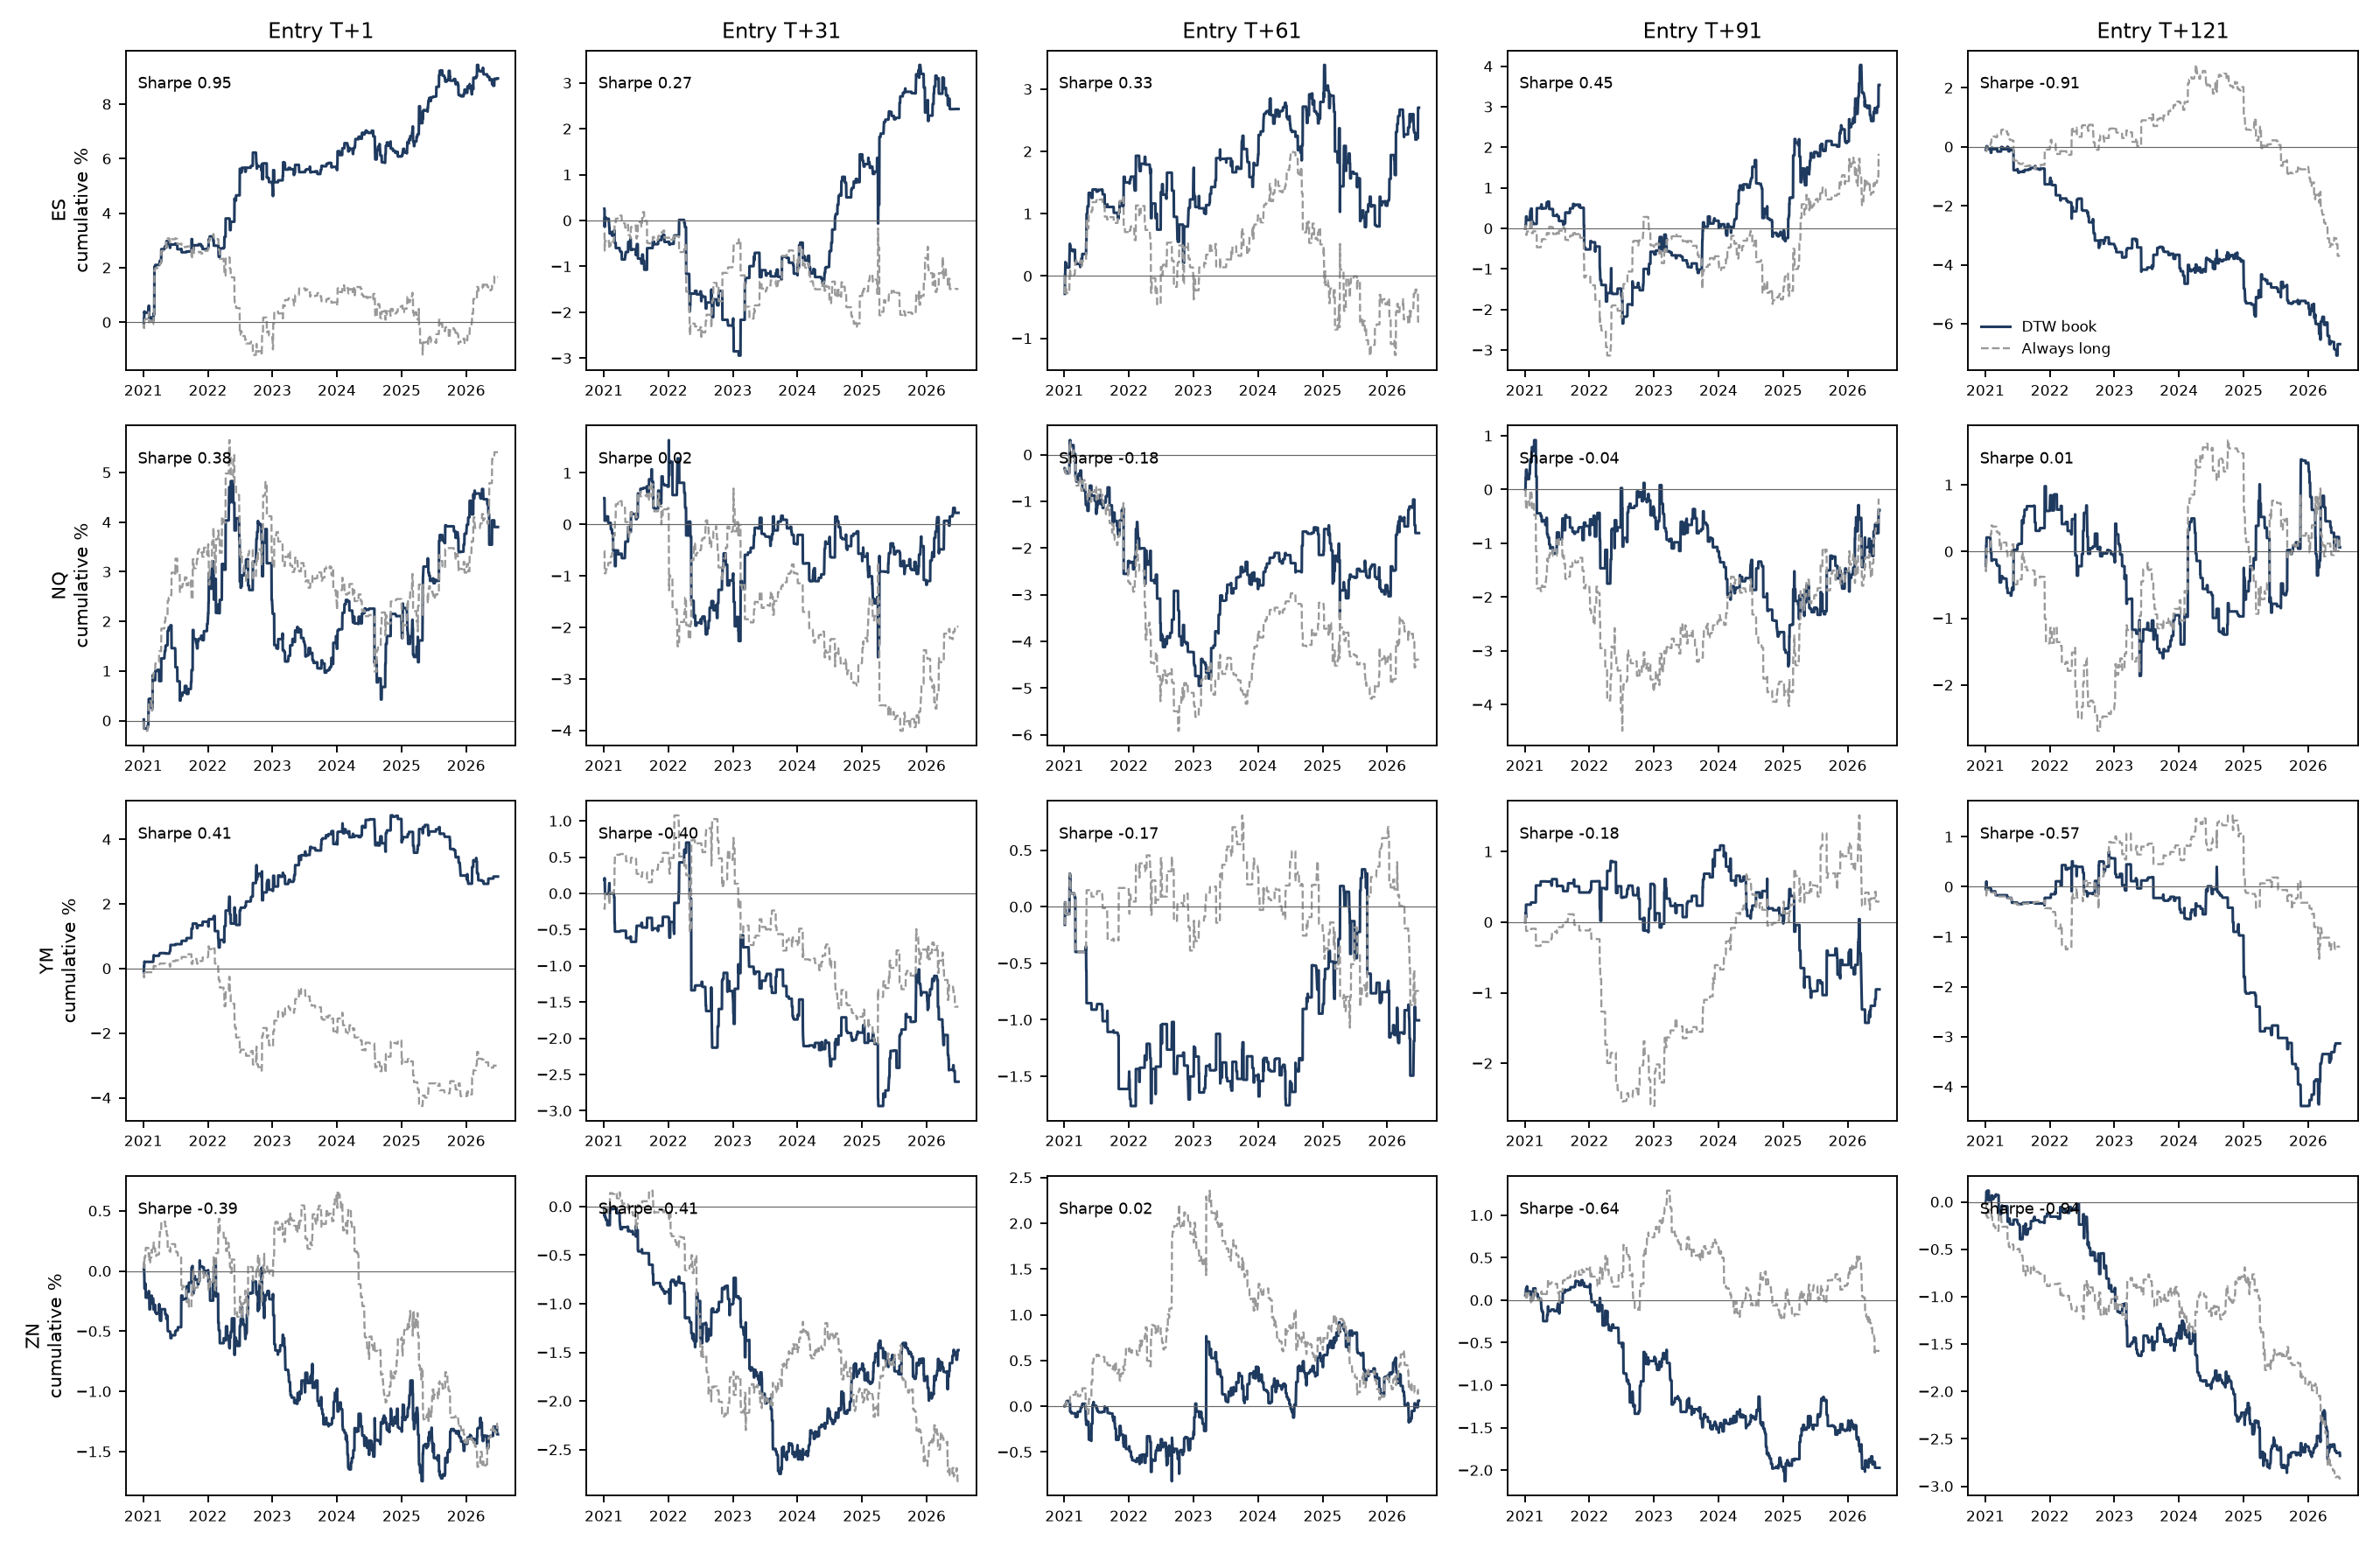
\includegraphics[width=0.72\linewidth]{pnl_curves_by_anchor_with_ym}
  \caption{Cumulative net P\&L at a quarter tick by window, 2021--2026, against always long in the
  same windows. Rows: \ES, \NQ, \YM, \ZN; columns: entry at $T+1$, $T+31$, $T+61$, $T+91$ and $T+121$.}
  \label{fig:byanchor}
\end{figure}

\subsection{2022 for equities}\label{sec:2022}

Table~\ref{tab:byyear} splits the test period by year. The \ES\ and equities books are positive
in five of six years; 2022, the year of the inflation shock and the fastest monetary tightening
in four decades, is the exception (equities $-0.87$, $-2.5\%$). A month-by-month breakdown shows
that 2022 was not a period of poor matches: the mean weighted similarity of the neighbours was
about 0.51 in \ES\ and 0.50 in \NQ\ in the first half of 2022, the same as in other years. In those
months the release windows themselves fell (about $-10$ bps on average in \ES\ and $-12$ bps in
\NQ), the \ES\ book was long in about 63\% of its trades, and the worst month, May, was a short
position into a rebound. The paths matched as closely as usual; what those paths had done next in
earlier years no longer held, because the market's reading of the same data had changed with the
Federal Reserve's reaction function. \YM\ moved the other way: it gained in 2022 (0.34) and lost
most in 2025. Win rates are 47--54\% in every year, so the edge, where it exists, comes from
winners being larger rather than more frequent.

\begin{table}[!tb]
  \centering\footnotesize
  \caption{Sharpe ratio by year, quarter tick per side.}\label{tab:byyear}
  \begin{threeparttable}
  \begin{tabular}{lcccccc}
    \toprule
    & 2021 & 2022 & 2023 & 2024 & 2025 & 2026 \\
    \midrule
    \ES & 0.67 & $-0.48$ & 0.89 & 1.33 & 0.76 & 1.27 \\
    \NQ & 0.12 & $-0.84$ & $-0.06$ & $-0.28$ & 0.94 & 1.36 \\
    \YM & $-0.23$ & 0.34 & 0.44 & $-0.28$ & $-1.67$ & $-0.61$ \\
    \ZN & $-1.24$ & $-1.01$ & $-1.73$ & $-0.52$ & $-0.25$ & $-0.89$ \\
    Equities (\ES\ + \NQ) & 0.71 & $-0.87$ & 0.70 & 0.78 & 1.04 & 1.58 \\
    \quad return & $+1.3\%$ & $-2.5\%$ & $+1.6\%$ & $+1.7\%$ & $+3.1\%$ & $+2.3\%$ \\
    \ES\ + \NQ\ + \YM & 0.46 & $-0.47$ & 0.80 & 0.49 & $-0.01$ & 1.16 \\
    Combined (\ES\ + \NQ\ + \ZN) & 0.71 & $-0.87$ & $-0.23$ & 0.77 & 1.03 & 1.57 \\
    \bottomrule
  \end{tabular}
  \begin{tablenotes}\footnotesize
    \item Notes: 2026 is a partial year (to June).
  \end{tablenotes}
  \end{threeparttable}
\end{table}

\subsection{Regime change for the 10-year}\label{sec:treasury_result}

\ZN\ went through a larger change of regime than the equity indices. Before 2021 policy rates
were near zero, \ZN's moves after releases were small, and a round trip at a quarter tick cost
13--21\% of its typical 30-minute move in every year. The 2022 tightening made rate news the
market's main driver and \ZN's post-release moves larger: the cost ratio fell from 17\% in 2021
to 15\% in 2022 and 10\% in 2023, before rising again to 12--17\% in 2024--2026. Before costs the
book does find something in \ZN: a gross Sharpe ratio of 0.34 and a small positive directional IC
(+0.016). But the regime change did not make the direction tradeable. In 2023, when the larger
moves let \ZN\ through the cost gate for part of the year, it lost, and the combined book scored
$-0.23$ that year against 0.70 for equities. \ZN\ loses in every test year at a quarter tick, its
strategy tracks being always long in the same windows ($-7.4\%$ for both), and it breaks even at
only 0.07 ticks per side. Without a gate, fixed equal-risk weights would have given \ZN\ 60\% of
the combined book at every cost and a Sharpe ratio of $-0.23$; the cost gate is what keeps the
combined book at 0.40. Bigger rate moves did not mean that the past paths forecast the next one:
in \ZN\ the tick is larger than the edge in any regime we observe.

\subsection{Against the surprise strategy}\label{sec:vs_surprise}

The natural competitor to the DTW book is a strategy that takes its direction from the consensus
surprise: buy after a release that beats the median forecast in the direction the market has
rewarded, sell after one that misses. Our companion study runs such books on the same four markets,
with the same releases, an entry one minute after the release and a 30-minute hold, over 2019--2026
and at a harsher cost of two ticks round trip plus \$4.50 in fees. It also runs a simple DTW-only
book at the first window and two books that trade only when the surprise and the DTW forecast agree.
These are not the ladder book of this paper---they use one window, a longer sample and a different
cost---but they show where the direction of the trade is best taken from.


\begin{figure}[!tb]
  \centering
  \begin{minipage}[t]{0.49\linewidth}\centering
    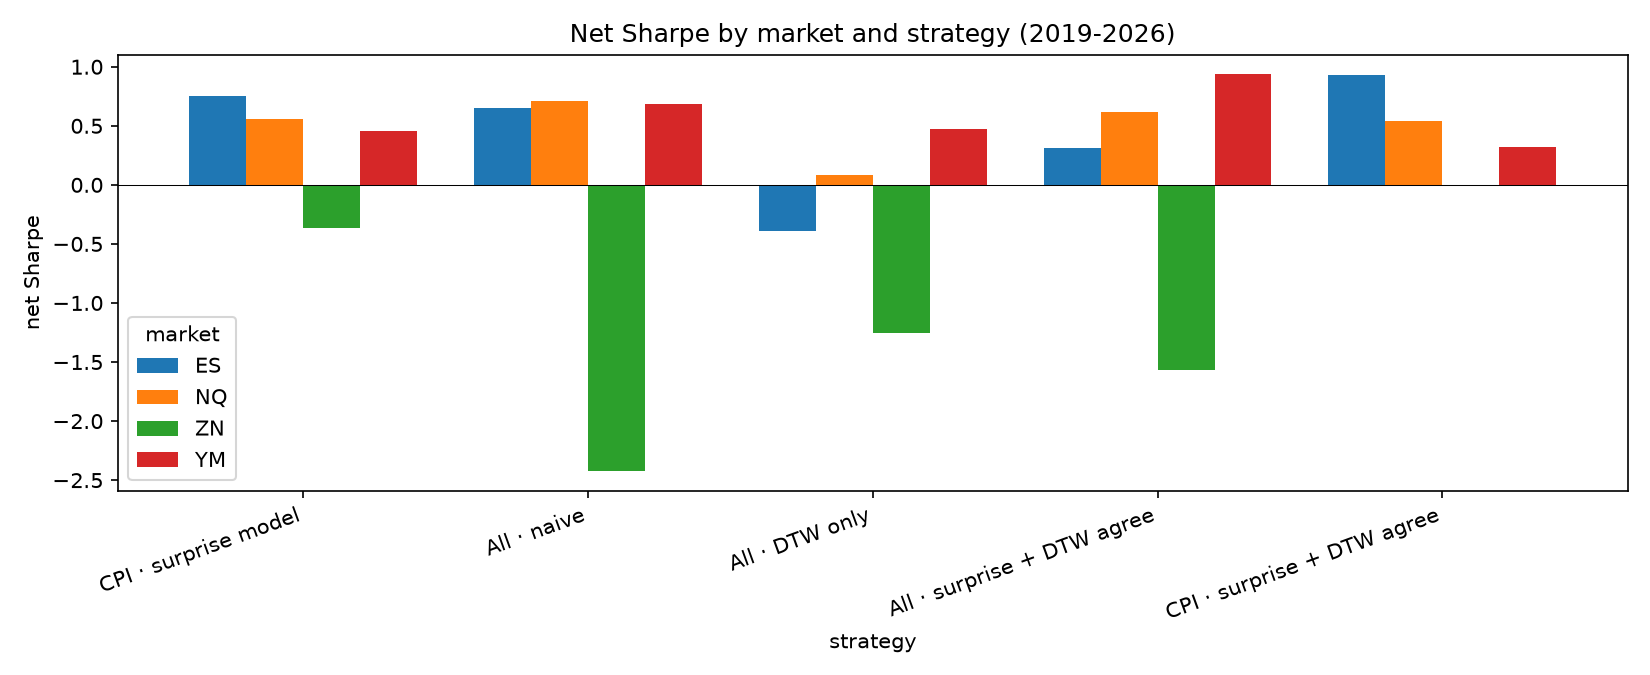
\includegraphics[width=\linewidth]{nb07b_sharpe_by_market}
    \caption{Net Sharpe ratio by market and strategy, 2019--2026, two ticks round trip plus \$4.50.
  ``All'': every release family that passes the impact screen; ``CPI'': CPI releases only;
  ``naive'': trade the sign of the surprise; ``surprise model'': trade a fitted drift forecast;
  ``DTW only'': trade the sign of the DTW forecast at the first window; ``surprise + DTW agree'':
  trade the surprise only when the DTW forecast has the same sign. \ZN\ has no CPI agree trades.}
    \label{fig:vs_surprise}
  \end{minipage}\hfill
  \begin{minipage}[t]{0.49\linewidth}\centering
    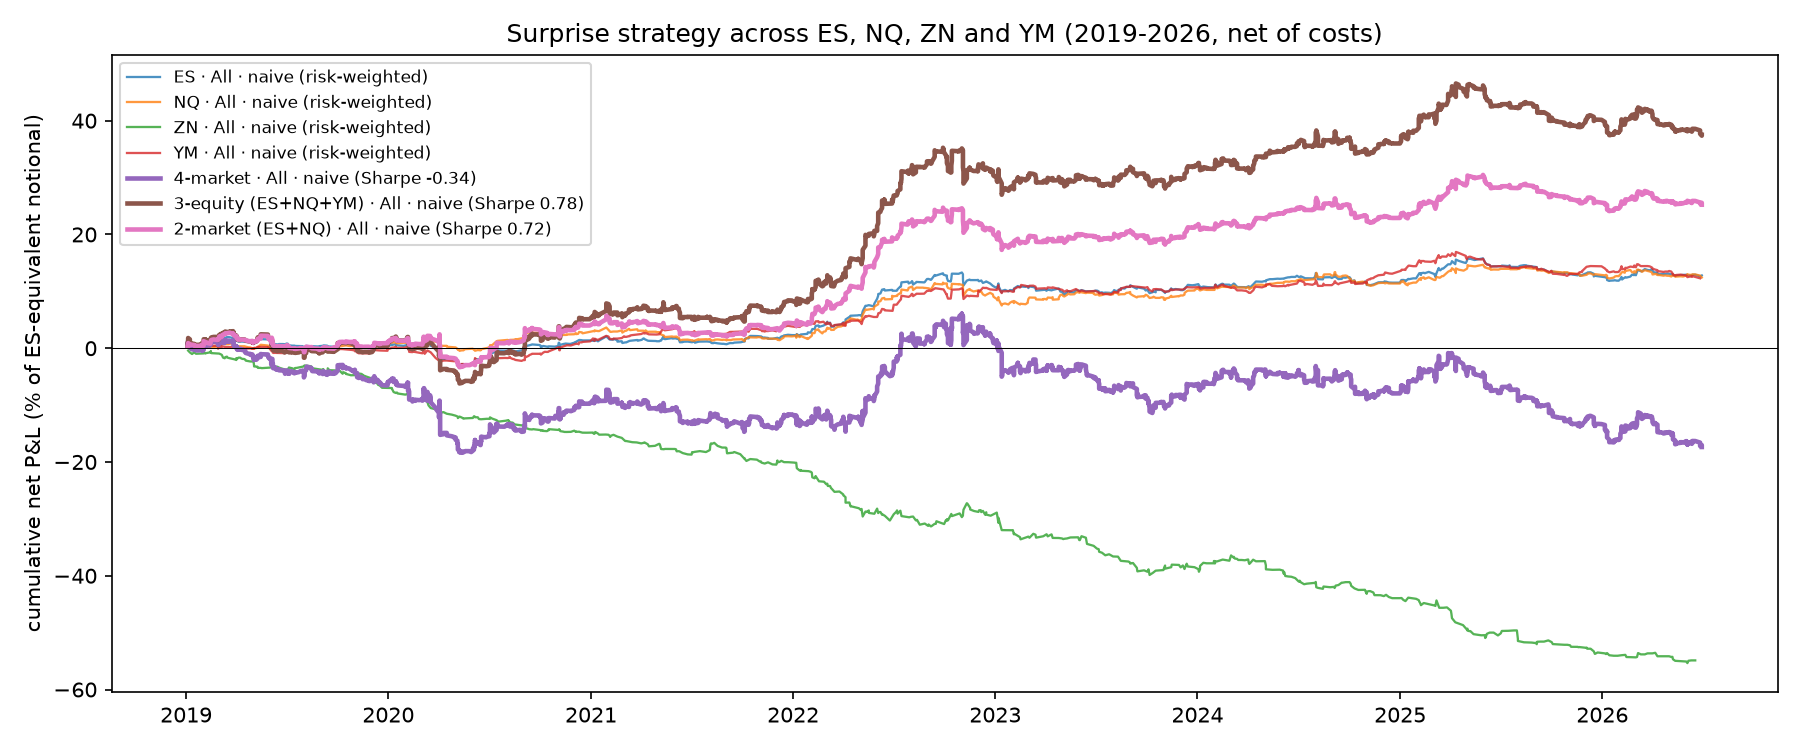
\includegraphics[width=\linewidth]{nb07b_portfolio_cumulative}
    \caption{Cumulative net P\&L of the broad surprise book (``All $\cdot$ naive'') by market,
  risk-weighted, and of the two-, three- and four-market portfolios with equal-risk weights fixed on
  2016--2018 (\ES\ 1.00, \NQ\ 0.71, \YM\ 1.02, \ZN\ 2.67), 2019--2026, net of costs.}
    \label{fig:vs_surprise_pnl}
  \end{minipage}
\end{figure}

Figure~\ref{fig:vs_surprise} gives the answer market by market. In all three equity indices the
broad surprise book earns about the same net Sharpe ratio, 0.65 in \ES, 0.71 in \NQ\ and 0.68 in
\YM, and the CPI surprise model earns 0.45--0.76. The DTW-only book is weaker in each: it loses in
\ES\ ($-0.39$), is flat in \NQ\ (0.08) and earns 0.47 in \YM. DTW adds most as a filter on the
surprise. Keeping only the trades on which the two agree raises the Sharpe ratio of the broad book
in \YM\ to 0.94 (0.94 also without 2022), and keeping only the CPI trades on which they agree raises
\ES's CPI book from 0.76 to 0.93, on fewer trades. In \ES\ the broad agree book is lower than the
surprise book alone (0.31), so the filter does not help everywhere. In \ZN\ every book loses after
costs, as in \ref{sec:treasury_result}: the broad surprise book goes from $-0.30$ before costs to
$-2.42$ after them.


Figure~\ref{fig:vs_surprise_pnl} combines the surprise books across markets. The three equity
books rise together, mostly in 2022, and the \ES\ + \NQ\ + \YM\ portfolio earns a Sharpe ratio of
0.78 (37.5\% in total) against 0.72 for \ES\ + \NQ. \ZN\ loses steadily, and because equal-risk
weights give it the largest weight, it turns the four-market portfolio negative ($-0.34$). Both
results match the DTW book: the equity indices carry the edge, adding \YM\ broadens the book, and
\ZN\ should be kept out at these costs. The comparison also locates the DTW book's role. As a
source of direction it is weaker than the surprise in every market; as a second opinion on the
surprise and as a book whose returns are nearly uncorrelated with it, it is useful.

Figure~\ref{fig:vs_surprise_cum} shows how these books earn over time, on all screened releases and
on CPI alone, and adds a fourth book that blends the two signals instead of requiring agreement.
In \ES\ and \NQ\ the surprise-only book is the highest curve on the broad set of releases, and the
DTW-only book drifts down in \ES\ from 2022 and goes flat in \NQ\ after 2023, the same break as in
\ref{sec:2022}. \YM\ is the one market where DTW adds to the surprise: the blend earns a Sharpe
ratio of 1.06 and the agree book 0.94, against 0.68 for the surprise alone, with a smoother path and
without the 2020 drawdown of the surprise book. On CPI the four books are close in every equity
index and most of their P\&L comes from 2022, so the CPI comparison rests on a single year. In
\ZN\ all four curves fall steadily; the surprise book falls most because it trades every release
and pays the cost each time.

\begin{figure}[!tb]
  \centering
  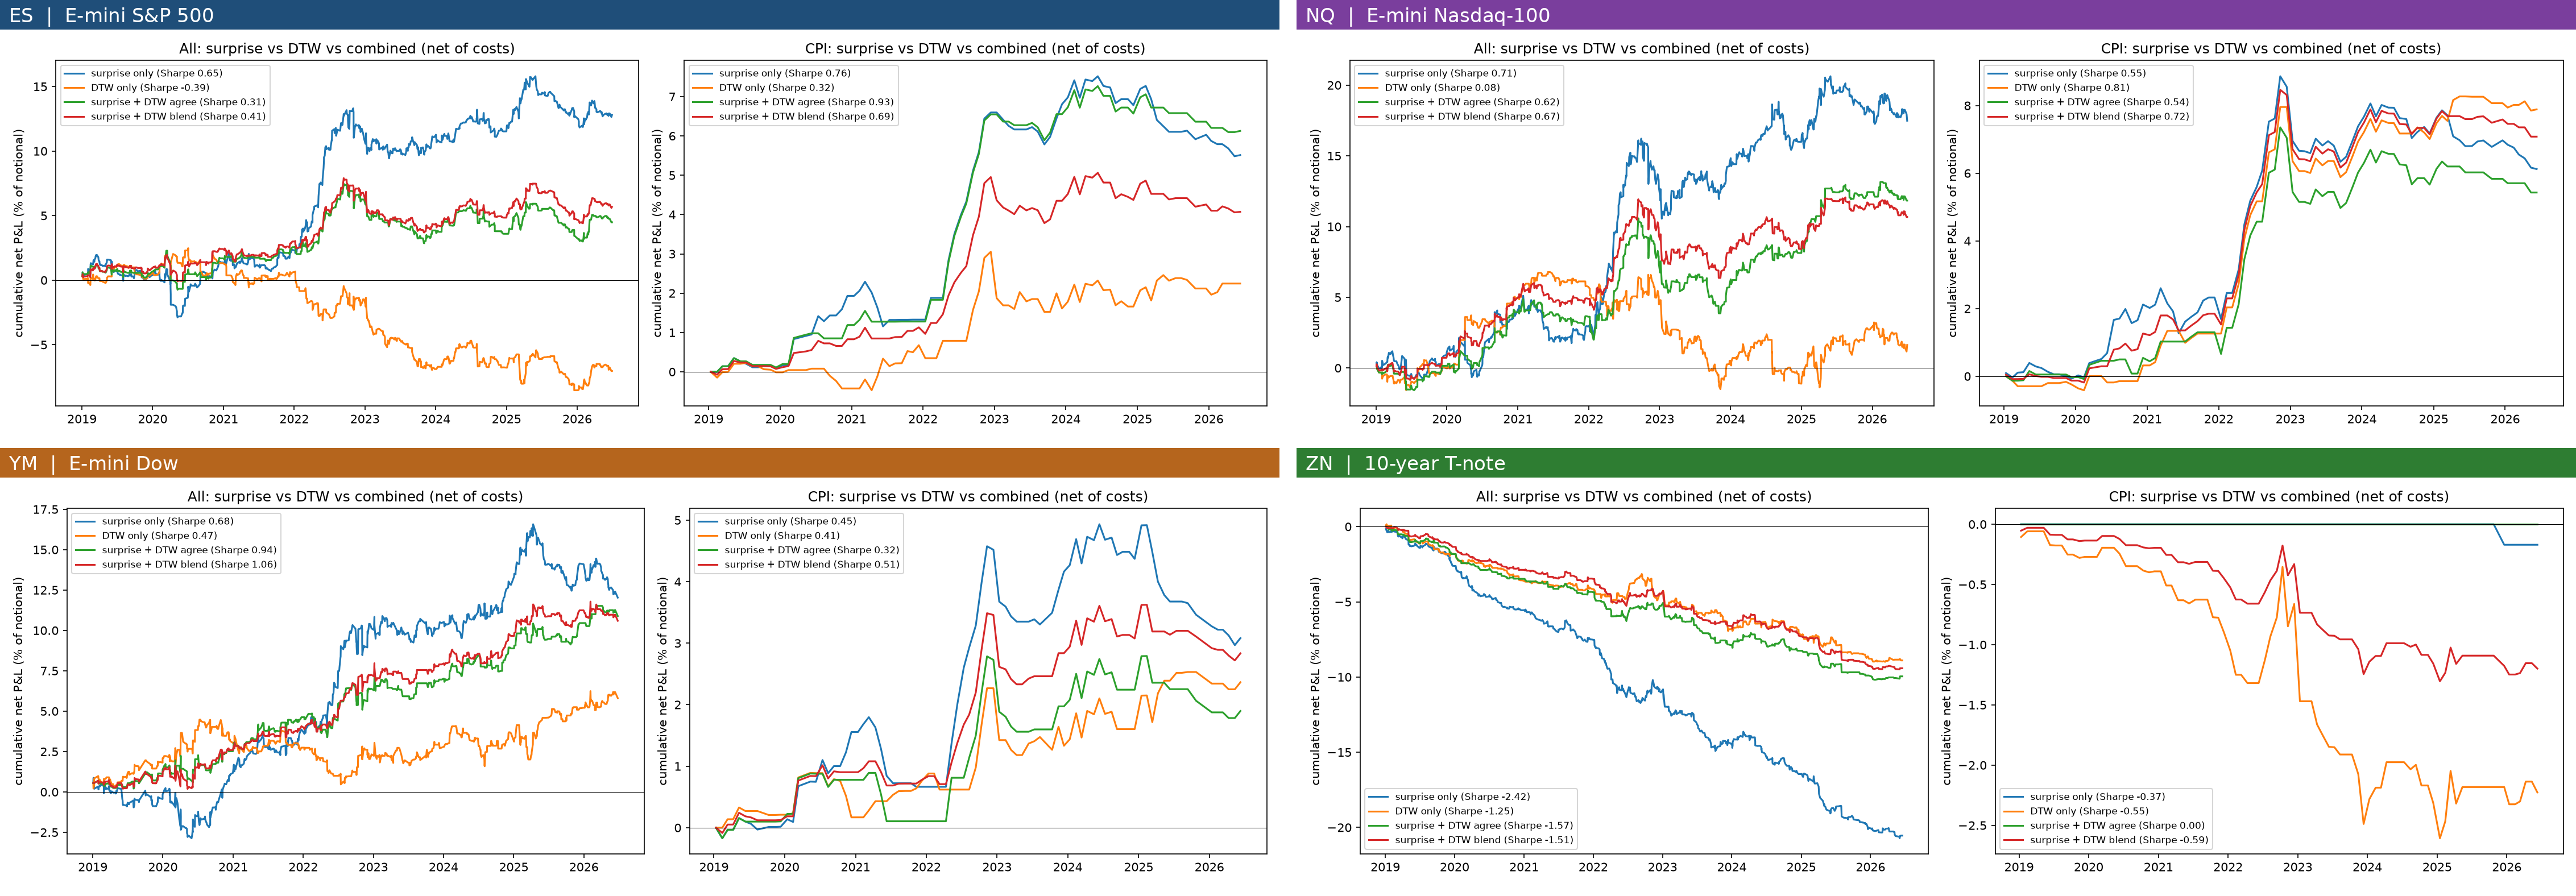
\includegraphics[width=\linewidth]{nb06_cumulative_2x2}
  \caption{Cumulative net P\&L, 2019--2026, two ticks round trip plus \$4.50, of four single-window
  books: surprise only, DTW only, surprise + DTW agree, and a blend of the surprise and DTW signals.
  For each market, left: all screened releases; right: CPI only. \ZN\ has no CPI agree
  trades (flat green line).}
  \label{fig:vs_surprise_cum}
\end{figure}

The surprise books above are built on the broad set of screened releases. Our first walk-forward
study instead trades only the three largest reports---CPI, Core PCE and payrolls---with five
rules: the naive sign of the surprise, a fitted surprise model, and three versions of that model
conditioned on the market's state before the release (volatility, momentum and the like). Every
slope, sign and state model is re-estimated on earlier releases only, and trades pay two ticks plus
\$4.50. On CPI
alone the naive sign is the best or close to the best in each equity index, with Sharpe ratios of
1.03 in \ES, 1.00 in \NQ\ and 0.99 in \YM, and conditioning on the state does not improve on it
by a significant margin. As in the DTW book, almost all of the gain comes in 2022. Adding PCE and payrolls lowers the naive rule to
0.33 in \ES\ and 0.38 in \NQ\ (0.57 in \YM). In \ZN\ the fitted models barely trade, because their forecast rarely exceeds a tick,
and the naive rule loses ($-0.05$ on CPI, $-0.65$ on the three reports). The surprise, in other
words, gives a better direction than the DTW analogues in the equity indices whether it is traded
on one report or many, and neither source survives the \ZN\ tick.



\FloatBarrier
\papersection{Conclusion}{sec:conclusion}

We asked whether the shape of the market's reaction to a scheduled macroeconomic release, matched
to earlier reactions with dynamic time warping, forecasts the next move in futures. Restricting
the library to post-release windows makes the method fast and gives every match a common cause,
and the answer has two parts.

The analogues forecast the size of the next move well. The dispersion of the neighbours' outcomes
ranks the absolute next return in every market and period, and sizing trades inversely to it
improves the \ES\ and equities books under every rule we tested.

The analogues forecast the direction of the next move only weakly, and not stably. Their
directional information coefficient was negative in 2013--2017 and positive afterwards. With the
setting and rule fixed in advance, the \ES\ book earns a Sharpe ratio of 0.64 at a quarter tick on
2021--2026, with no market beta, a drawdown of $-5\%$, a direction that beats random signs and a
timing that passes a leak test; the equities book earns 0.54. But \NQ\ earns only 0.11, \YM---run
through the same pipeline as an out-of-sample market---loses, and the \ES\ result ranges from 0.17
to 0.64 across reasonable constructions. The edge sits in the first window after the release, the
2022 loss came from a change in what similar paths did next rather than from poor matches, and in
\ZN\ the larger moves of the new rate regime still left the edge below one tick.

Three conclusions follow for practice. First, anchoring to scheduled events and entering only
after the release are what make a path-based method testable at all. Second, DTW is best used for
what it measures robustly---the size and uncertainty of the next move---while the direction comes
from a source with a clearer economic link, such as the consensus surprise, with which the DTW
book is nearly uncorrelated and which it improves as a filter in \YM\ and in \ES's CPI trades
(\ref{sec:vs_surprise}). Third, before any capital is committed, the book needs recorded fills
in the minutes after releases, because slippage decides whether a per-trade edge of this size
survives. Natural extensions are a book that trades only the first window, averaging the
forecasts of the best settings, and a direction signal that combines the surprise with the shape
of the reaction.


\enlargethispage{2\baselineskip}
\begingroup\footnotesize\setlength{\bibsep}{0pt}
\IfFileExists{aea.bst}{\bibliographystyle{aea}}{%
  \IfFileExists{chicago.bst}{\bibliographystyle{chicago}}{\bibliographystyle{apalike}}}
\bibliography{references}
\endgroup

\end{document}
